\chapter{姿态} \label{chap:chap36}

姿势的控制涉及两个相互关联的目标,平衡和定向,这对日常生活中的大多数任务至关重要。
平衡控制使身体保持稳定平衡,避免跌倒。
方向使身体部分相对于彼此和与世界对齐,例如保持头部垂直。
平衡和方向都使用几种不同类型的控制:
自动姿势反应、预期姿势调整、站立时的姿势摇摆、身体图式的感觉整合、垂直方向和步态期间的动态稳定性。


要了解保持平衡和方向的复杂性,请想象您正在游船上等候餐桌。
你有一个装满饮料的托盘,要送到滚动甲板另一侧的桌子上。
即使你的大脑忙于记住顾客的命令,用于控制姿势定向和平衡的无意识但复杂的感觉运动过程也会让你以有效和协调的方式四处走动而不会摔倒。
当您穿过滚动甲板时,您的大脑会迅速整合和解释感官信息并调整运动输出以保持您的平衡以及头部和躯干的直立方向,并稳定支撑全副眼镜托盘的手臂。
船的突然意外运动会引起自动姿势反应,从而防止跌倒。在伸手将玻璃杯放在桌子上之前,神经系统会做出预期的姿势调整以保持平衡。


整合了体感、前庭和视觉信息,以提供身体在空间中相对于支撑面、重力和视觉环境的位置和速度的连贯感。
由于地表不稳定且视觉无法提供地球稳定的信息,因此您对前庭信息的依赖性比平时更大。
您的头部保持稳定,而您的躯干运动和步行模式会根据移动表面引起的不平衡进行调整。
你注意到当你试图同时完成这两个目标时,你的自主任务和平衡控制都会恶化。



\section{平衡和定向是姿势控制的基础}

姿势平衡是指通过抵抗作用于身体的外力来主动稳定上半身的能力。
虽然影响地球平衡的主要外力是重力,但也必须抵抗其他惯性力和外部扰动。
根据特定的任务或行为,不同组的肌肉会在响应或预期平衡受到干扰时被激活。


姿势定向是指身体各部分(例如躯干和头部)相对于彼此和环境主动对齐的能力。
根据特定的任务或行为,身体部分可能与重力垂直线、视觉垂直线或支撑面对齐。
例如,在下坡滑雪时,头部可能会朝向重力和惯性垂直方向,但不会朝向倾斜的视觉或支撑面参考。


姿势控制的生物力学要求取决于解剖结构和姿势方向,因此因物种而异。
然而,在各种物种中,姿势平衡和定向的控制机制具有许多共同特征。
姿势控制的感觉运动机制在人类和四足哺乳动物中非常相似,尽管它们的习惯性姿势不同。



\subsection{姿势平衡控制身体的重心}

由于许多节段由关节连接,身体在机械上不稳定。
为了保持平衡,神经系统必须控制身体质心的位置和运动以及身体围绕它的旋转。
质心是代表身体总质量的平均位置的点。
以站立的成年人为例,重心位于第二腰椎前方约 2 厘米处;
在年幼的孩子中,它更高。
质心的位置不是固定的,而是取决于姿势方向。
例如,当您在站立时弯曲髋关节时,重心会从身体内部的位置移动到身体外部的位置。


尽管重力会拉动所有身体部分,但对身体平衡的净影响是通过身体的质心起作用的。
重力引起的力与脚和地面之间的力相反。
表面上的每个点都会在脚上产生一个力。
作用在脚和地面之间的所有力可以加起来产生一个单一的力向量,称为地面反作用力。
表面上地面反作用力向量的原点是脚上所有力的旋转效应平衡的点,称为压力中心(方框~\ref{box:36_1})。



\begin{proposition}[神经解剖学导航术语] \label{box:36_1}
	
	\quad \quad \textit{压力中心}定义为支撑表面上地面反作用力向量的原点。为了使身体处于静态平衡状态,即保持静止,重力和地面反作用力产生的力必须相等且相反,\textit{压力中心}必须直接位于\textit{质心}下方(图~\ref{fig:36_1}A)。
	\textit{质心}和\textit{压力中心}的错位会导致\textit{质心}的运动。
	例如,如果\textit{质心}投影到支架底部的方向是\textit{压力中心}的右侧,则身体将向右摆动,直到\textit{压力中心}向右移动,以将\textit{质心}移回支架底部。
	
	\quad \quad 然而,站立从来都不是真正静止的。
	当身体运动(姿势摆动)时,\textit{质心}和\textit{压力中心}不对齐,动态平衡必须保持平衡(图~\ref{fig:36_1}B)。
	事实上,当身体不受支撑时,\textit{压力中心}和\textit{质心}会持续运动,很少对齐,尽管在安静的姿势下随着时间的推移取平均值时,它们是重合的。
	安静站立期间身体的摆动可以通过\textit{质心}或\textit{压力中心}随时间的轨迹来描述,例如摆动路径,面积,速度和频率。
	
	\quad \quad 在步行、跑步、转弯和跳跃等更具活力的情况下,即使\textit{质心}短暂超出支撑基础,也可以实现稳定性。
	例如,当单腿站立或站在窄梁上时,可以利用旋转髋关节,手臂和其他身体部位或\textit{压力中心}运动产生的动量来改变地面反作用力的方向,使身体\textit{质心}返回其支撑底座以保持稳定性(图~\ref{fig:36_1}B)。
	如果\textit{质心}位于支撑底部之外并远离它,则受试者可能需要迈出一步或抓住一个稳定的物体来改变支撑底部并避免摔倒。
	
\end{proposition}


\begin{figure}[htbp]
	\centering
	\includegraphics[width=0.66\linewidth]{chap36/fig_36_1}
	\caption{通过移动压力中心来控制质心。
		A. 重力引起的力通过躯干中的\textit{质心}。 
		表面对每只脚施加向上的力,使得地面反作用力向量起源于支撑表面上的\textit{压力中心}。 
		下图:即使脚保持原位,\textit{压力中心}(蓝色位移)和 \textit{质心}(金色位移)也会随着我们摇摆而运动。
		在双脚正常站立期间,身体\textit{质心}的投影保持在支撑底部(与地面接触的脚周围的浅蓝色矩形)内以达到平衡。
		站立的人的支撑基础由脚在支撑表面上的接触来定义。
		B. 在动态情况下,例如单腿站在窄梁上,即使身体\textit{质心}位移(黄金位移)短时间超出支撑底部,也可以保持平衡。
		上下半身反向旋转等策略可以倾斜地面反作用力,从而使身体\textit{质心}加速回到其支撑基础之上\cite{otten1999balancing}。}
	\label{fig:36_1}
\end{figure}


站立时保持平衡需要将重心向下投射到支撑底部,这是一个由与环境接触的身体部位定义的假想区域。
例如,站立的人的两只脚或一只脚定义了支撑基础(方框~\ref{box:36_1})。
然而,当站立的人靠在墙上或用拐杖支撑时,支撑的基础从脚下的地面延伸到身体与墙壁或拐杖之间的接触点。
因为身体总是在运动,即使在稳定的姿势下,身体的质心也会相对于支撑点不断移动。
姿势不稳定性取决于质心加速朝向和超出其支撑底部边界的速度以及身体质心的向下投影与边界的距离有多近。


直立姿势需要两个动作:
(1)通过将质心保持在一定高度和关节稳定来保持对重力的支撑,以及(2)通过控制质心在水平面上的轨迹来保持平衡。
平衡和抗重力支持分别由神经系统控制,在某些病理条件下可能受到不同的影响。
例如,当中风后出现痉挛或脑瘫肌张力减退时反重力支持可能过度,尽管平衡控制可能得以保留。
或者,在前庭疾病中,尽管平衡控制紊乱,但反重力支持可能是正常的。


反重力支撑或“姿势张力”是由肌肉的强直激活提供的,这些肌肉产生对地面的力,以保持躯干和四肢伸展,并将重心保持在适当的高度。
在人类中,大部分抵抗重力的支撑是由关节(例如膝盖)中的被动骨对骨力提供的,膝盖可以在站立期间完全伸展,以及拉伸的韧带(例如髋关节前部的韧带)。
然而,人类的反重力支持也需要主动强直肌肉收缩,例如脚踝、躯干和颈部伸肌。
然而,姿势张力不应被视为肌肉激活的静态状态,如去大脑强直或帕金森病强直等病理学中所见。
正常的姿势基调不断变化,就像“波浪”或“风中的芦苇”,以适应姿势调整、\textit{自主运动}和任务要求的变化。


然而,姿势张力不足以保持平衡。
双足动物和四足动物本质上都是不稳定的,它们的身体在静止站立时会摇晃。
主动收缩的肌肉表现出类似弹簧的刚度,有助于抵抗身体摇摆,但仅靠肌肉刚度不足以保持平衡。
即使通过肌肉收缩来加强四肢也不足以控制平衡。
相反,肌肉激活的复杂模式会产生方向特定的力来控制身体的重心。
即使是细微的运动引起的身体摇摆,例如呼吸时胸部的运动,也会被姿势张力的改变所积极抵消。



\subsection{姿势定向能预示平衡障碍}

姿势定向是身体各部分相对于彼此和环境对齐的方式。 动物通过调整身体姿态来高效完成特定任务。
尽管这种姿势定向与平衡控制相互作用,但这两个系统可以独立运作。
例如,足球守门员可能会牺牲保持平衡的目标,通过调整身体姿势来拦截球。
相比之下,患有帕金森病或胸椎后凸畸形的患者可能会使用低效的弯曲姿势来保持站立时对平衡的有效控制。


在一段时间内保持身体姿势所需的能量会影响姿势定向。例如,在人类中,躯干相对于重力的直立方向最大限度地减少了力,从而最大限度地减少了将身体的质心保持在支撑底部上方所需的能量。
任务要求也会影响姿势定向。
对于某些任务,重要的是稳定身体在空间中的排列,而对于其他任务,则有必要使一个身体部位相对于另一个部位保持稳定。
例如,当拿着满满的玻璃杯走路时,重要的是要稳定手以抵抗重力以防止溢出。
相比之下,边走边看手机时,手必须相对于头部和眼睛保持稳定,以保持视力。


受试者可能会采用特定的姿势定向来优化有关身体运动的感觉信号的准确性。
例如,当在船内站立和行走时,表面和视觉参考可能不稳定,有关地球垂直度的信息主要来自前庭输入。
当在不稳定的表面上保持平衡时,一个人通常会根据重力垂直方向对齐头部,因为当头部直立且稳定时,垂直方向的感知最为准确。


习惯性身体方向的预期改变可以最大限度地减少可能的干扰的影响。
例如,人们通常会向预期的外力方向倾斜,或者在预期稳定性会受到影响时弯曲膝盖、张开站姿并伸展手臂。



\section{姿势反应和预期姿势调整使用模式化的策略和协同作用}

当突然的干扰导致身体摇摆时,会使用各种姿势运动策略来将重心保持在支撑底部。
在一种策略中,支撑底部相对于支撑面保持固定:当脚保持在原位时,身体围绕脚踝旋转回到直立位置(图~\ref{fig:36_2})。
在其他策略中,支撑的基础被移动或扩大,例如,通过迈出一步或用手抓住支撑(图~\ref{fig:36_2}B)。


\begin{figure}[htbp]
	\centering
	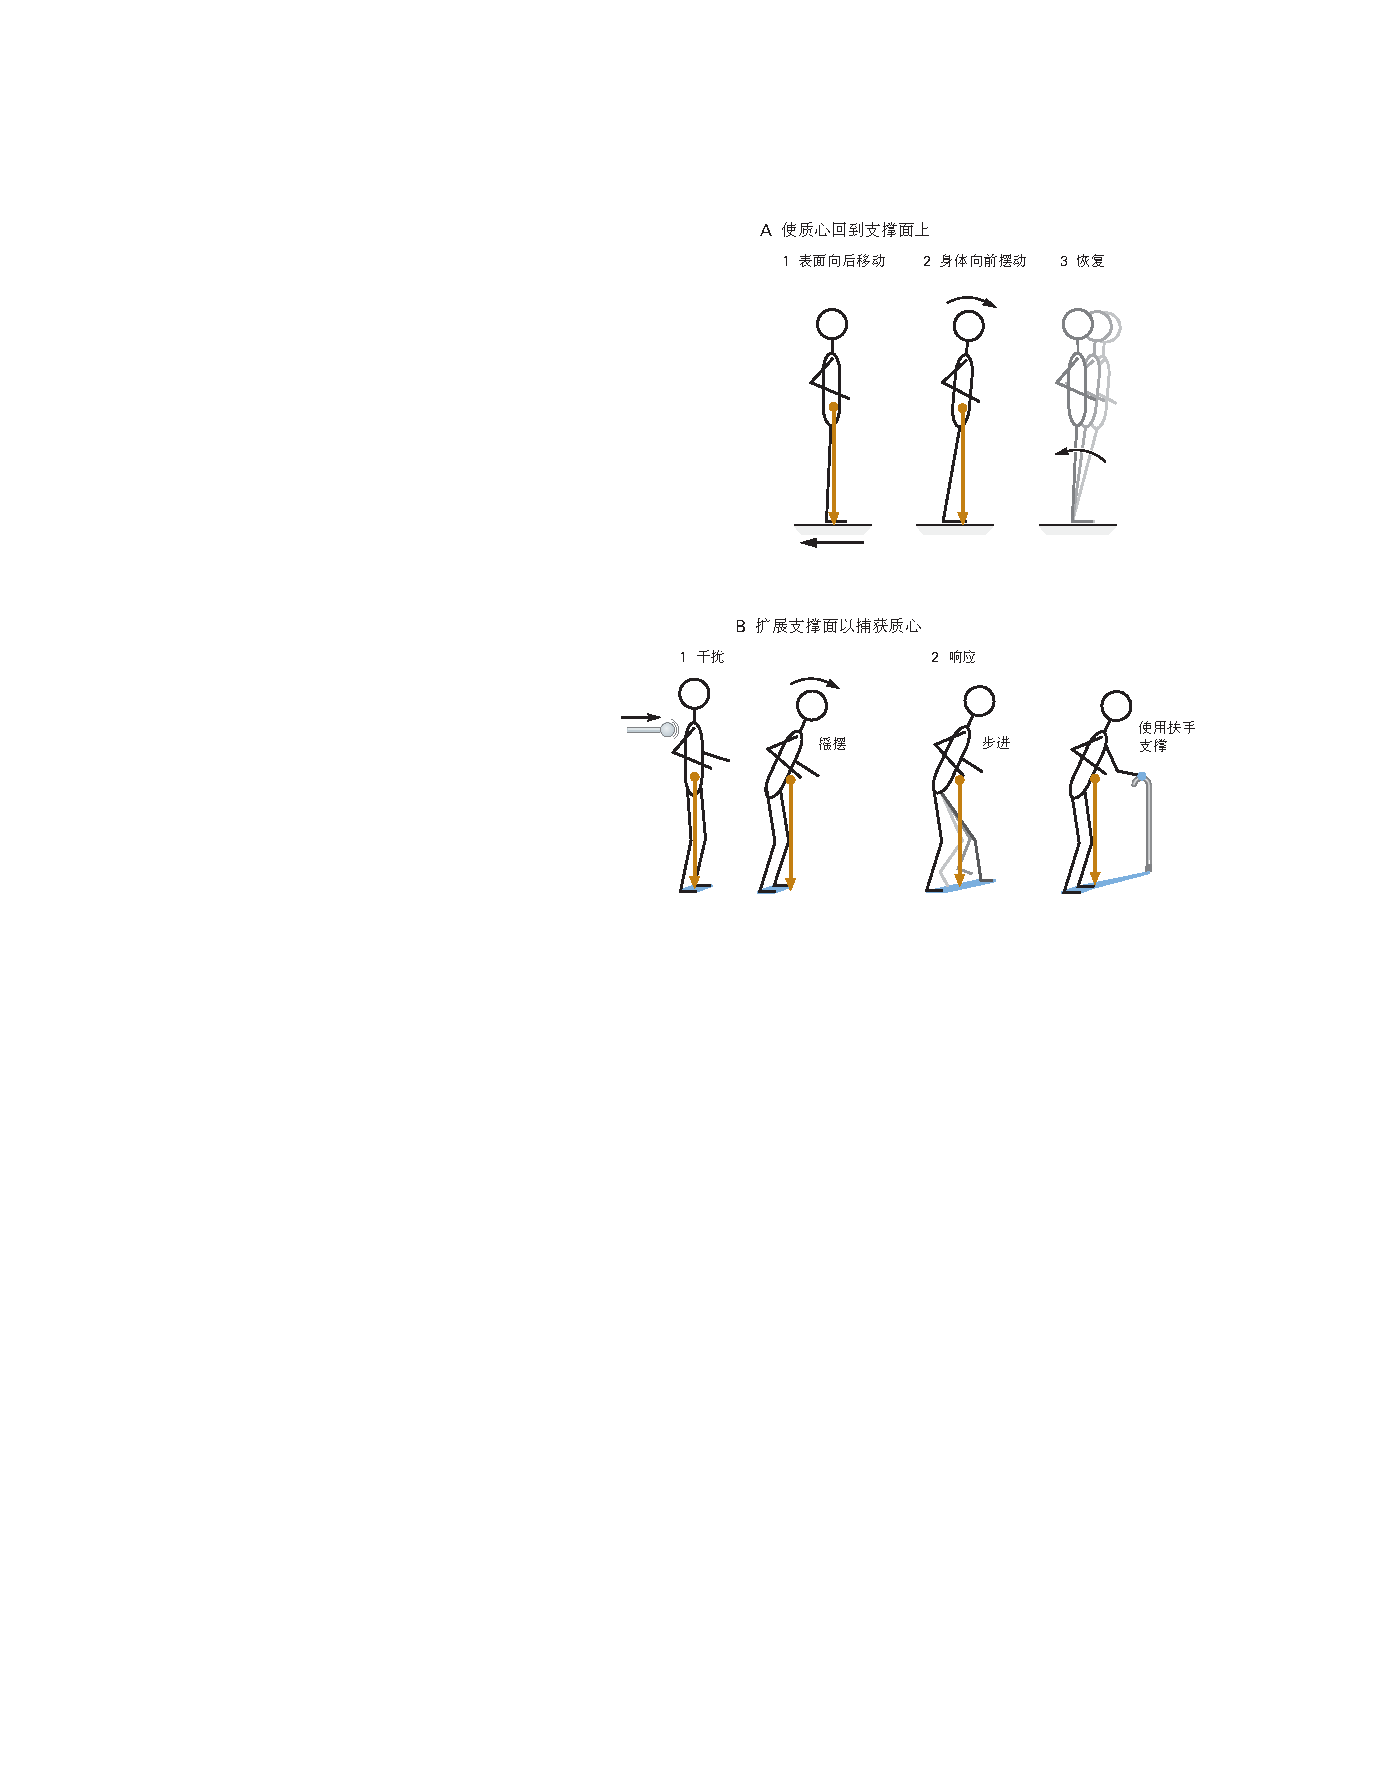
\includegraphics[width=1.0\linewidth]{chap36/fig_36_2}
	\caption{自动姿势反应将\textit{质心}保持在\textit{支撑面}内。
		A. 一种恢复平衡的姿势策略是将质心带回到支撑基础上的原点。
		当受试者站立的平台突然向后移动时,身体向前摇摆,质心的投影向脚趾移动。
		在恢复过程中,身体会主动向脚踝周围的表面施加力,使重心回到脚上的原始位置。
		B. 另一种姿势策略扩大了支撑基础,以将重心保持在基础内。
		干扰导致受试者向前摇摆,质心向支撑底部的边界(地面上的蓝色区域)移动。
		底座可以通过两种方式扩大:
		迈出一步并将脚放在重心前面以减慢身体的运动,或者抓住一个支撑物,从而扩展底座以包括手和支撑物之间的接触点。}
	\label{fig:36_2}
\end{figure}


旧的运动控制观点将躯干和近端肢体肌肉作为主要的姿势效应器。
最近的行为研究表明,根据与环境接触的身体部位和平衡的生物力学要求,来自颈部和躯干、腿部和手臂或脚部和手部的任何肌肉群都可以充当姿势肌肉。


在研究姿势控制系统时,科学家们以可控的方式破坏平衡,以确定受试者的自动姿势反应。
这种反应由地面反作用力向量、压力中心的运动和身体部位的运动来描述。
许多肌肉的电活动由\textit{肌电图}记录,它反映了支配骨骼肌的$ \alpha $ 运动神经元的放电,从而为了解神经系统的平衡控制输出提供了一个窗口。
所有这些测量的组合使研究人员能够推断出平衡控制背后的活跃神经过程。



\subsection{自动姿势反应补偿突然的干扰}

对突然干扰的自动姿势反应不是简单的牵张反射,而是一组肌肉以保持平衡为目标的特征序列的协同激活。
也就是说,用于姿势反应的肌肉募集服务于平衡的要求,而不是由干扰引起的肌肉长度的反射性变化。
例如,当人脚下的表面在脚尖朝上的方向上旋转时,踝关节伸肌(腓肠肌)被拉长,可能会出现轻微的牵张反射。
然而,平衡的姿势反应募集拮抗踝屈肌(胫骨前肌),其本身因表面旋转而缩短,同时抑制腓肠肌的拉伸反应。
相比之下,当平台向后移动时,腓肠肌再次延长,但现在它募集募用于姿势反应,牵张反射后肌电图活动的第二次爆发证明了这一点。
因此,由扰动引起的肌肉长度的初始变化并不能确定该肌肉是否被用于姿势控制,并且牵张反射不是姿势控制的基础。
事实上,单突触牵张反射太弱,无法有效地移动身体重心,而且经常被激活以恢复平衡的姿势肌肉没有被拉伸。


对突然干扰的自动姿势反应具有特有的时间和空间特征。 在障碍开始后,必须迅速募集肌肉的姿势反应。
站立的猫下方支撑面的突然移动会在 40 到 60 毫秒内引起\textit{肌电图}活动(图~\ref{fig:36_3})。
人类的姿势反应潜伏期较长(脚踝肌肉为 90-120 毫秒);
增加的延迟归因于人类更大的体型,因此从感觉受体到中枢神经系统再到腿部肌肉的信号传导距离更大。
自动姿势反应的潜伏期比自主反应时间短,但比单突触牵张反射长。


\begin{figure}[htbp]
	\centering
	\includegraphics[width=1.0\linewidth]{chap36/fig_36_3}
	\caption{自动姿势反应具有模式化的时间特征。
		\textit{肌电图}活动具有典型的潜伏期。
		在平台加速开始约 40 毫秒(人类为 100 毫秒)后,平台的前向运动在猫的髋伸肌(前股二头肌)中引起\textit{肌电图}反应。
		这种潜伏期是模式化的,并且在受试者之间是可重复的,大约是单突触牵张反射的四倍。
		当平台移动时,爪子向前移动,而躯干由于惯性而留在后面,导致重心相对于平台以越来越快的速度向后移动。
		随着肌肉激活后\textit{地面反作用力的水平分量}增加,质心的速度达到峰值然后下降。
		肌电图活动开始和主动反应开始之间大约 30 毫秒的延迟反映了兴奋-收缩耦合和肌肉骨骼顺应性。
		自动姿势反应伸展后肢,推动躯干向前并恢复重心相对于爪子的位置。}
	\label{fig:36_3}
\end{figure}


涉及支撑基础变化的姿势反应,例如踏步,比脚保持原位时发生的反应有更长的延迟。
较长的时间可能为通过皮层的长循环传输的命令提供了更大的灵活性;
例如,开始迈步的脚的选择、迈步的方向以及迈步绕过障碍物的路径。


姿势肌的激活导致肌肉收缩和力量的发展,导致关节处的扭矩(旋转力)。
最终结果是主动响应,即地面反作用力(方框~\ref{box:36_1}),它将重心恢复到其在支撑底座上方的原始位置(图~\ref{fig:36_3})。
肌电图激活和主动反应之间的延迟,猫大约 30 毫秒,人类大约 50 毫秒,反映了每块肌肉的兴奋-收缩耦合时间以及肌肉骨骼系统的顺应性。


特定肌肉中\textit{肌电图}活动的幅度取决于姿势障碍的速度和方向。
幅度随着站立的人或猫下方的可移动平台速度的增加而增加,并且随着平台运动方向的系统变化而以单调方式变化。
每块肌肉都对一组有限的扰动方向做出响应,并具有特征调谐曲线(图~\ref{fig:36_4})。



\begin{figure}[htbp]
	\centering
	\includegraphics[width=0.81\linewidth]{chap36/fig_36_4}
	\caption{自动姿势反应具有模式化的方向特征\cite{macpherson1988strategies}。
		A. 猫的臀中肌(髋关节伸肌和外展肌)对水平面上的一系列运动方向做出反应。
		此处显示的肌电图\textit{肌电图}记录来自一只站在平台上的猫,该平台在 16 个均匀间隔的方向中的每个方向上在水平面上移动。 
		左后肢的臀中肌被几个方向(粉红色)的运动激活,并在其余方向(灰色)受到抑制。 
		垂直虚线表示平台加速的开始。 
		中间是\textit{肌电图}活动幅度与自动姿势反应期间运动方向的极坐标图;
		它代表肌肉的定向调谐曲线。
		在响应的前 80 毫秒期间,根据曲线下的面积计算\textit{肌电图}振幅。 
		B. 每块肌肉都有一个不同于其他肌肉的特征性定向调谐曲线,即使它们具有相似的动作。
		例如,中间股二头肌和颅半膜肌都是髋关节的伸肌。}
	\label{fig:36_4}
\end{figure}


尽管单个肌肉具有独特的定向调谐曲线,但肌肉并不是独立激活的,而是协同激活的,具有典型的时间延迟。
协同作用中的肌肉在姿势反应期间接收到共同的命令信号。
通过这种方式,身体的许多肌肉仅由几个信号控制,减少了计算适当姿势反应所需的时间(方框~\ref{box:36_2})。


\begin{proposition}[肌肉的协同激活] \label{box:36_2}
	
	\quad \quad 协调的运动需要精确控制身体的许多关节和肌肉。
	维持控制在生物力学上是复杂的,部分原因是关节旋转和肌肉激活的不同组合可以实现相同的目标。
	这种冗余赋予了极大的灵活性,例如,在修改步进模式以跨越我们道路上的障碍时,但代价是大脑对运动轨迹和力的计算变得更加复杂。
	
	\quad \quad 运动指令的计算必须包括许多因素,包括重力等外力的影响以及一个身体部分在运动过程中对另一个身体部分施加的力。
	当大脑计算对突然干扰的姿势反应时,所有这些因素都会发挥作用,但在计算上还有一个额外的时间限制:反应必须在一定时间内发生,否则就会失去平衡。
	
	\quad \quad 长期以来,人们一直认为大脑通过将控制变量分组来简化对运动的控制,例如,将几块肌肉激活在一起。
	使用将复杂数据解析为少量组件的数学技术,可以确定,在对平台运动的多个方向进行自动姿势反应期间,只需要四个协同作用就可以解释人类腿部和躯干13块肌肉的绝大多数激活模式(图~\ref{fig:36_5})。
	每种协同作用的激活都会产生一个独特的地面力方向,这表明姿势控制是基于与任务相关的变量,例如脚与地面之间的力,而不是单个肌肉的收缩力。
	
	\quad \quad 就像和弦中音符的排列一样,每个肌肉协同作用指定了特定肌肉与其他肌肉一起激活的时间和幅度。
	正如一个音符属于几个不同的和弦一样,每一块肌肉都属于不止一种协同作用。
	当几个和弦同时演奏时,和弦结构在众多的音符中不再明显。
	类似地,当几个协同作用同时激活时,观察到的肌肉模式会出现非结构化的复杂性,但是特定肌肉的激活是系统添加协同命令的结果。
	协同作用的同时激活简化了运动的神经命令信号,因为只需要几个中央命令,而不是每个肌肉单独的命令,同时允许姿势控制的灵活性和适应性。
	
\end{proposition}


\begin{figure}[htbp]
	\centering
	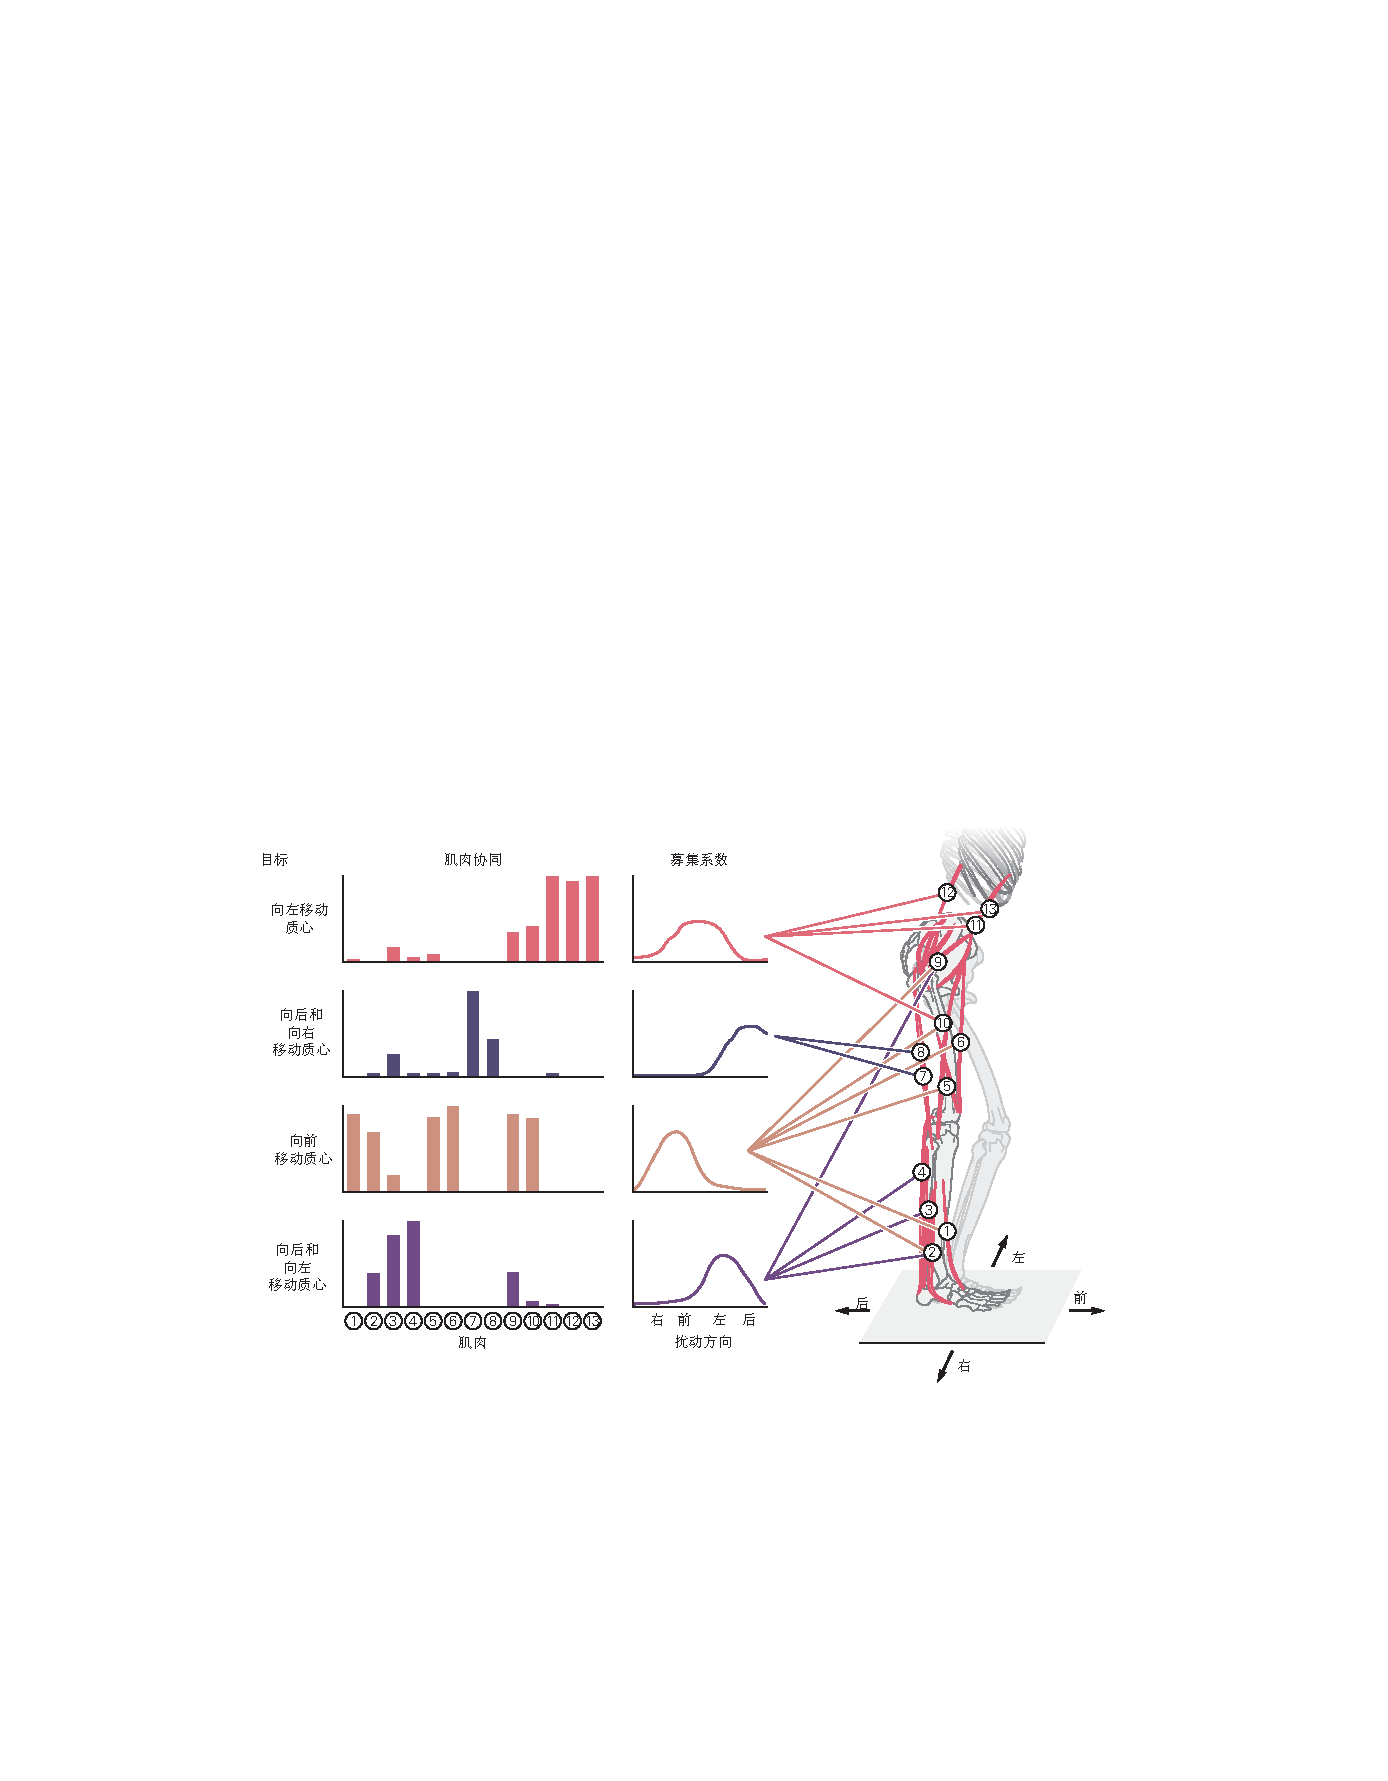
\includegraphics[width=1.0\linewidth]{chap36/fig_36_5}
	\caption{姿势指令激活协同效应,而不是单个肌肉。
		几个肌肉的协同激活可以将运动目标转化为特定的肌肉激活模式。
		每一种肌肉协同作用都会以固定的比例激活一组肌肉(彩色条),以产生实现姿势目标所需的机械输出。
		每个小节的高度代表每个肌肉的相对激活量或权重(1-13)。
		在由中央命令和感觉驱动(募集功能)驱动的行为过程中,每一种协同作用或多或少在特定时间被激活。
		例如,不同的姿势协同作用在不同的跌倒方向上被激活。}
	\label{fig:36_5}
\end{figure}


在对扰动的姿势响应中募集的一组肌肉取决于身体的初始姿势。
如图~\ref{fig:36_6}A~所示,同样的扰动会导致一个人在没有帮助的情况下站立、抓住稳定的支撑物站立或四肢蹲伏时产生截然不同的姿势响应。
例如,在自由直立站立期间,向前摇摆会激活腿后部和躯干的肌肉。
当受试者抓住稳定的支撑物时,首先激活手臂的肌肉而不是腿部的肌肉。
当受试者像猫一样用脚趾和手指蹲伏时,腿前部和手臂的肌肉会被激活。


\begin{figure}[htbp]
	\centering
	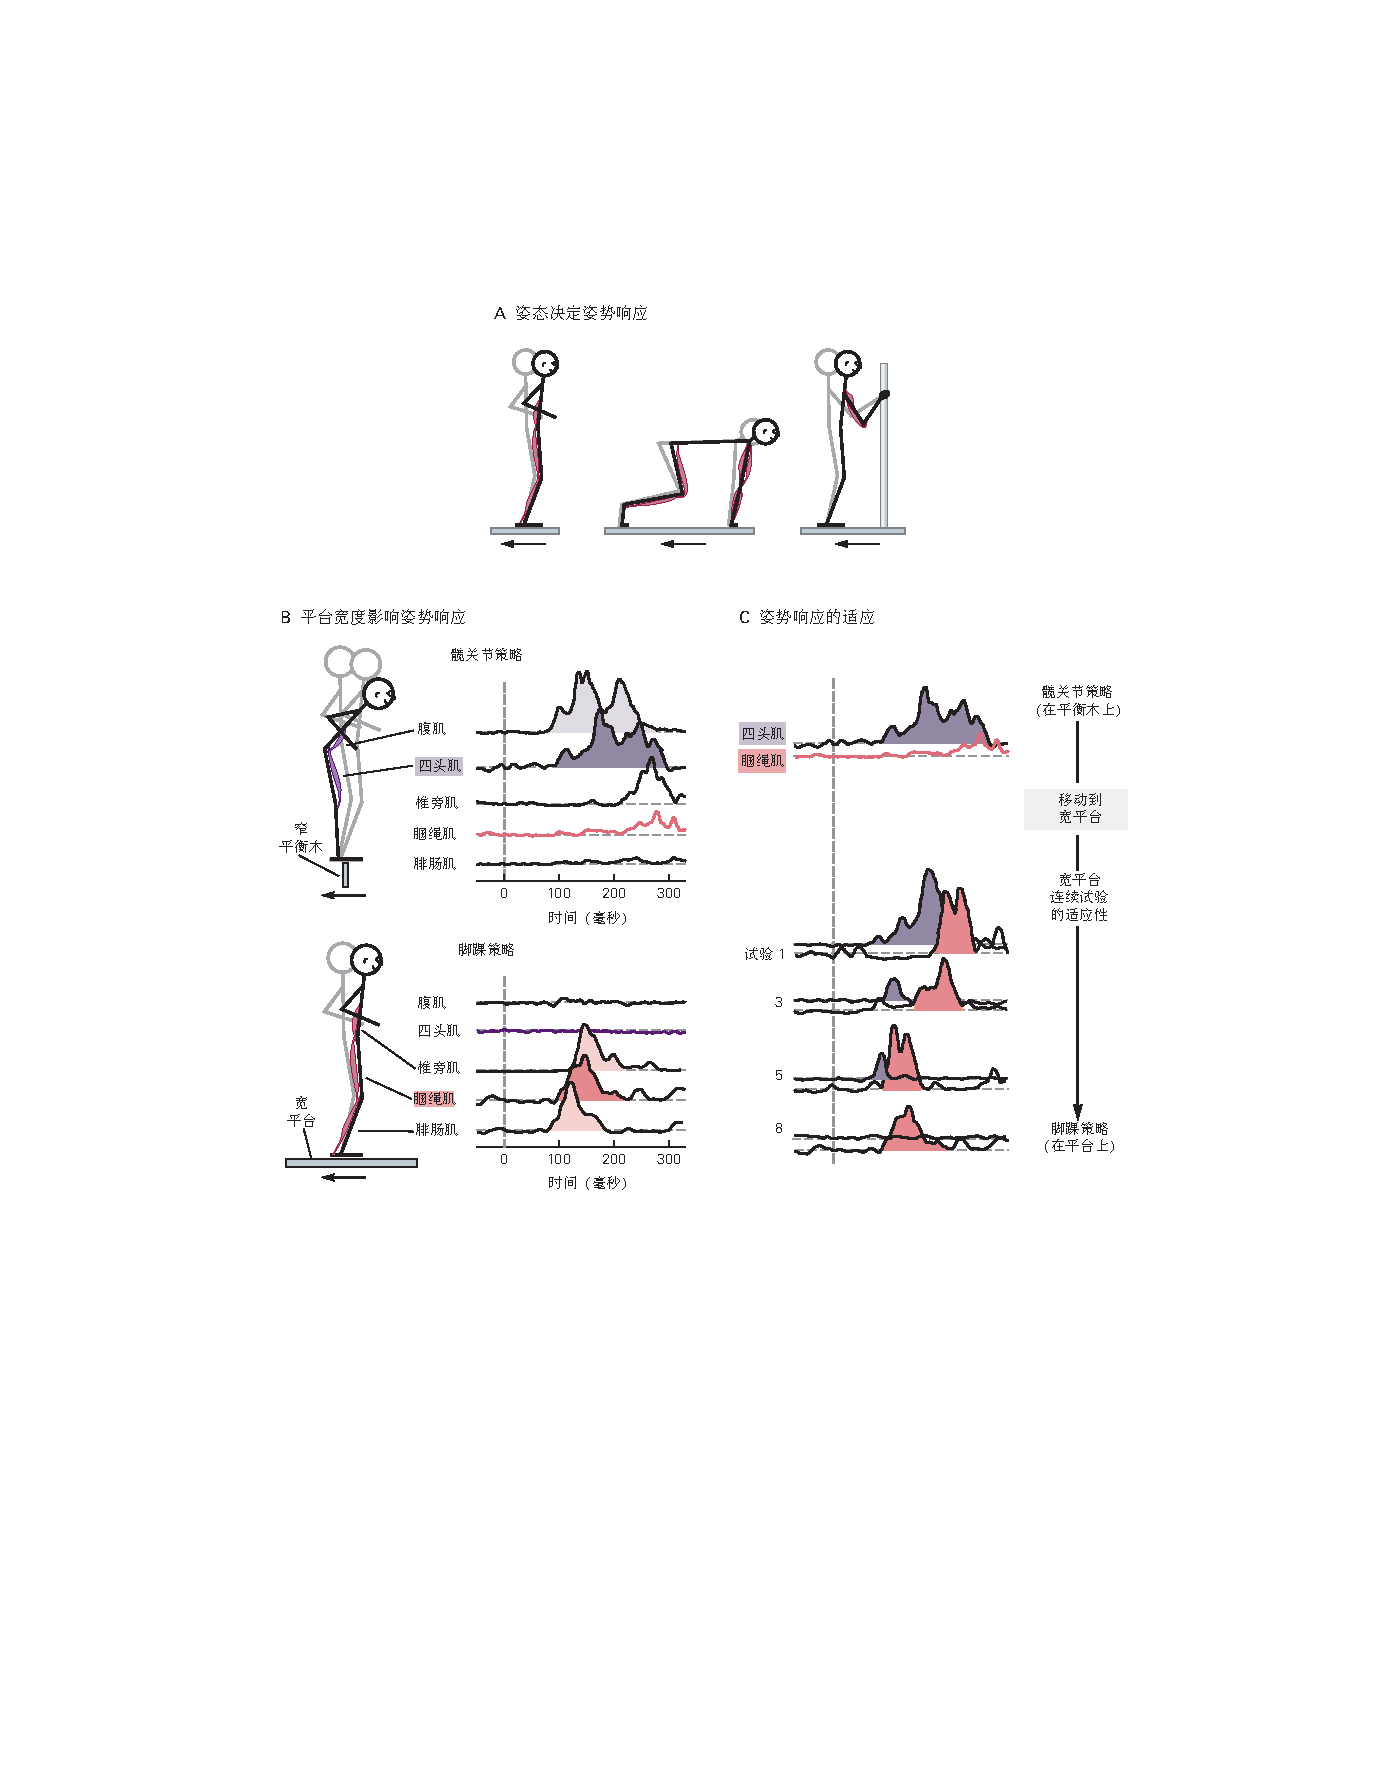
\includegraphics[width=1.0\linewidth]{chap36/fig_36_6}
	\caption{自动姿势响应随生物力学条件而变化。
		A. \textit{平台的向后运动}会根据初始姿势激活不同的肌肉群。
		灰色简笔画显示初始位置(无支撑直立、四足支撑或直立支撑)。
		在每个姿势响应中激活的肌肉以红色显示\cite{dunbar1986neural}。
		B. 当受试者站在一根突然向后移动的\textit{窄平衡木}上时,前部肌肉(\textit{腹肌}和\textit{四头肌})被募集来弯曲躯干,并伸展脚踝,向后移动髋关节(\textit{髋关节策略})。
		当受试者站在一个向后移动的\textit{宽平台}上时,他的后部肌肉(\textit{椎旁肌}、\textit{腘绳肌}和\textit{腓肠肌})会被激活,通过旋转脚踝使身体恢复直立姿势 (\textit{脚踝策略})。
		代表不同姿势响应的肌肉以颜色突出显示。
		图中的垂直虚线表示平台(或平衡木)加速的开始。
		C. 受试者从窄平衡木移动到宽平台后姿势策略适应。
		在平衡木上,股四头肌被激活,腘绳肌沉默;
		适应宽平台后,观察到相反的情况。
		从股四头肌到腘绳肌激活的转变发生在一系列试验中;
		股四头肌的活动幅度逐渐减小,而腘绳肌被激活的时间越来越早,直到试验 8,股四头肌的活动完全消失。
		脚踝和躯干肌肉表现出相似的适应模式\cite{horak1986central}。}
	\label{fig:36_6}
\end{figure}


由于姿势响应受最近经验的影响,它们只能逐渐适应新的生物力学条件。
当受试者站立的平台向后运动引起向前摇摆时,脚踝、膝盖和髋关节的后部肌肉在平台开始移动后 90 毫秒开始依次激活。
这种姿势响应,即\textit{脚踝策略},主要通过围绕踝关节旋转身体来恢复平衡。
然而,当窄梁的向后运动引起前摇时,仅靠表面扭矩是不可能恢复平衡的,并且髋关节和躯干的前部肌肉会被激活。
这种姿势反应,即\textit{髋关节策略},通过在髋关节处向前弯曲并在脚踝处反向旋转来恢复身体的重心(图~\ref{fig:36_6}B)。


当受试者从站在宽阔的平台上移动到狭窄的平衡木上时,她或他在前几次试验中坚持使用\textit{脚踝策略}。
当站在平衡木上时,此策略不起作用,受试者会倒下。
经过几次试验,受试者将逐渐转向使用\textit{髋关节策略}。
类似地,从平衡木移回平台需要多次试验以使姿势反应适应\textit{脚踝策略}(图~\ref{fig:36_6}C)。


尽管在受试者从平衡木移动到地面后感觉刺激会立即发生变化,但姿势反应会逐渐调整,因为它会通过反复试验调整为最佳行为。
如果姿势反应是简单的反射,它们会在感觉驱动发生变化时立即发生变化。
姿势行为的反复试验变化通常发生在潜意识水平(内隐学习),涉及更新右顶叶皮层内的身体图式和内部世界模型。
这种身体模式是动态的,因为它会根据经验不断更新。


姿势响应不仅会随着练习而改善,而且会保留这种改善,这是运动学习的标志。
例如,当受试者练习站在振动表面上时,他们会逐渐学会减少质心位移的程度,并且大部分这种改善在第二天得以保留(图~\ref{fig:36_7})。
患有神经系统疾病(例如多发性硬化症或帕金森氏病)的患者,其姿势响应明显受损,通常可以通过练习来改善他们的姿势控制,尽管他们可能需要比平时更多的练习才能保持这种改善(图~\ref{fig:36_7})。


\begin{figure}[htbp]
	\centering
	\includegraphics[width=0.85\linewidth]{chap36/fig_36_7}
	\caption{可以通过练习学习和保留姿势响应。
		A. 身体质心的位移(\textit{质心},金黄色的振荡线)响应不同振幅(灰色)的向前和向后平台振荡,作为健康受试者学习减少姿势不稳定性。
		B. 在第 1 天的训练课程中,前向-后向表面振荡引起的身体\textit{质心}位移减少,并且这种改善在健康对照受试者的第 2 天得到保留。
		多发性硬化症患者也学会减少\textit{质心}位移,但第二天不会保持这种改善。
		比较增益(\textit{质心}/表面位移)的组变化的平均值和标准误差\cite{gera2016postural}。}
	\label{fig:36_7}
\end{figure}



\subsection{预期姿势调整补偿\textit{自主运动}}

\textit{自主运动}也会破坏姿势方向和平衡。
例如,站立时快速向前抬起手臂会产生伸展髋关节、弯曲膝盖和背屈脚踝的力量,使身体的重心相对于脚向前移动。
神经系统提前了解\textit{自主运动}对姿势对齐和稳定性的影响,并激活预期的姿势调整,通常在主要运动之前(图~\ref{fig:36_8}A)。


\begin{figure}[htbp]
	\centering
	\includegraphics[width=1.0\linewidth]{chap36/fig_36_8}
	\caption{预期的姿势调整先于自主运动。
		A. 随拉力的增加,手臂自主拉动的姿势成分在振幅和提前时间上增加。
		在这个实验中,受试者被要求拉动用电线连接在墙上的把手。
		受试者站在测力板上,并在收到信号后快速拉动手柄以达到指定的峰值力,该峰值力在最大拉力的 5\% 到 95\% 之间变化。
		每次拉动之前都会激活腿部肌肉,从而在踝关节周围产生旋转力或扭矩。
		拉力越大,脚踝扭矩越大越早。
		轨迹在时间为零时手柄上拉力开始时对齐\cite{lee1990organization}。
		B. 姿势调整仅在需要时伴随\textit{自主运动}。
		与 A 部分一样,受试者被要求拉动固定在墙上的把手。
		肌电图轨迹在零时间对齐,即手臂肌肉(肱二头肌)开始活动。
		在无支撑站立期间,腿部肌肉(\textit{腘绳肌}和\textit{腓肠肌})先于手臂肌肉被激活,以防止身体在手臂拉动过程中向前旋转。
		红色箭头表示腿部腓肠肌激活的开始,灰色箭头表示手臂肱二头肌的激活。
		当受试者的肩部由一根刚性杆支撑时,预期的腿部肌肉活动就没有必要了,因为身体无法向前旋转。
		当不需要预期的姿势肌肉活动时,手臂激活会更早。
		阴影区域表示预期的姿势响应(红色)和初始手臂肌肉激活(棕色)\cite{cordo1982properties}。
		C. 在步行过程中,\textit{质心}的轨迹由脚部放置控制。
		身体的重心在双脚之间,随着受试者向前行走而向前和左右移动。
		当身体仅由一条腿支撑时(单支撑阶段),\textit{质心}位于支撑底部之外并向举重肢移动。
		人们在行走时不会跌倒,因为脚在下一步上的放置会使\textit{质心}减速并将其推回中线\cite{mackinnon1993control}。}
	\label{fig:36_8}
\end{figure}


预期的姿势调整特定于生物力学条件。
当一个自由站立的受试者快速拉动固定在墙上的把手时,腿部肌肉(腓肠肌和腿筋)会先于手臂肌肉被激活(图~\ref{fig:36_8}B)。
当受试者的肩膀靠在一根刚性杆上进行同样的拉动时,不会发生预期的腿部肌肉活动,因为神经系统依赖杆的支撑来防止身体向前移动。
当响应外部提示拉动手柄时,手臂肌肉在支撑状态下比在独立状态下激活得更快。
因此,当任务需要主动的姿势稳定性时,自主的手臂肌肉激活通常会延迟。


另一种常见的预备姿势调整发生在一个人开始走路时。
通过减轻一条腿的重量,重心向前加速和横向加速。
这种姿势调整似乎独立于作为持续运动基础的步进程序(第~\ref{chap:chap33}~章)。
类似地,重心向前移动先于用脚尖站立。
如果受试者只是简单地激活小腿肌肉而不向前移动他的重心,他就无法保持站立状态;
在重力恢复扁平足姿势之前,他只是暂时抬起脚趾。
在激活小腿肌肉之前,将重心向前移动到脚趾上方,使其与预期的支撑基础对齐,从而稳定脚趾的姿势。


自主运动期间的姿势平衡不仅需要控制身体质心的位置和运动,还需要控制围绕质心的角动量。
潜水员在空中时可以围绕质心进行精细的翻滚和扭转,尽管一旦他离开板子,他的质心轨迹就固定了。
在\textit{自主运动}期间,姿势调整通过预测旋转力来控制身体的角动量。



\subsection{姿势控制与运动相结合}

在行走和跑步过程中,身体处于不断下降的状态,因为重心向前和横向移向处于摆动阶段的腿(图~\ref{fig:36_8}C)。
在行走过程中,仅当双脚着地时,重心才位于支撑底部内,即双支撑阶段,这仅为步态周期的三分之一。
当一只脚支撑身体时,重心在脚前移动,始终位于支撑底部的内侧。


在行走和跑步过程中,通过将支撑底座向前和横向移动到落下的重心下方,可以防止跌倒。
步态期间的姿势平衡依赖于每一步的位置来控制质心的速度和轨迹。
神经系统使用有关地形和周围环境的视觉信息提前几个步骤来计划脚的放置。


行走期间的主要姿势挑战是控制移动腿上的上半身重心,尤其是在横向方向上。
躯干的过度横向位移和过度的横向足部放置可变性是运动期间姿势不稳定的迹象。
步态期间姿势稳定性异常的患者可能仍然表现出正常的自动和预期姿势调整、不同感觉条件下的姿势摆动和垂直方向,这表明姿势控制和步态具有不同的神经系统回路。



\section{必须整合和解释体感、前庭和视觉信息以保持姿势}

由于来自任何一个感觉系统的运动信息可能是模糊的,因此必须将多种模式整合到姿势中心以确定身体的哪种方向和运动是合适的。
任何一种模式对姿势控制系统的影响都因任务和生物力学条件而异。


根据流行的理论,感觉方式被整合以形成位于顶叶皮层内身体的内部表征,神经系统使用顶叶皮层来计划和执行运动行为。
随着时间的推移,这种内部表征必须适应与早期发育、衰老和受伤相关的变化。



\subsection{体感信号对于自动姿势响应的时间和方向很重要}

许多类型的体感纤维触发并塑造自动姿势响应。
I 组中最大的纤维(直径 12-20 微米)似乎对正常响应延迟至关重要。
I 组纤维破坏后\textit{肌电图}响应的延迟时间更长、上升时间更慢以及幅度更低反映了由肌梭初级受体编码的加速度信息的丢失(图~\ref{fig:36_9}A)。
最大和最快传导的感觉纤维是来自肌梭的 Ia 传入神经和来自高尔基腱器官的 Ib 传入神经,以及一些来自皮肤机械受体的纤维(第~\ref{chap:chap18}~章)。
I 组纤维提供有关身体生物力学的快速信息,包括对肌肉拉伸、肌肉力量和脚底定向特定压力的响应。
然而,来自肌梭和皮肤受体的 II 组纤维也可能在塑造自动姿势响应中发挥作用。
尽管它们可能太慢而无法生成响应的最早部分,但它们可能会对质心速度和位置进行编码。


\begin{figure}[htbp]
	\centering
	\includegraphics[width=0.63\linewidth]{chap36/fig_36_9}
	\caption{大直径体感纤维的缺失会延迟自动姿势响应。
		在维生素 B$_6$ 中毒破坏全身的大直径(I 组)体感纤维之前和之后,记录了猫对可移动平台水平运动的姿势响应的\textit{肌电图}。
		运动神经元和肌肉力量不受体感纤维损失的影响,但有关肌肉长度和力量的传入信息会减少。
		A. 在 I 组纤维破坏后,支撑平台的水平运动引起的臀中肌姿势响应显著延迟。
		这种大约 20 毫秒的延迟会导致共济失调和难以保持平衡。
		B. I 组纤维的破坏延迟了后肢的激活。
		这种延迟减缓了\textit{质心}的恢复和平台位移后平衡的恢复。
		\textit{地面反作用力的水平分量}开始延迟导致\textit{质心}的峰值位移更大,并延迟其返回相对于爪子的原点。}
	\label{fig:36_9}
\end{figure}


本体感受和皮肤输入都提供有关姿势方向的线索。
例如,在直立姿势期间,随着身体在重力作用下摇摆,肌肉会伸长和缩短,从而产生与负荷、肌肉长度和伸展速度相关的本体感受信号。
关节受体可以检测关节上的压力,而脚底的皮肤受体对压力中心的运动和身体摇摆时地面反作用力角度的变化做出响应。
肾脏附近的压力受体对重力(体重力感受)敏感,神经系统利用它来帮助检测直立或倾斜的姿势。
所有这些信号都有助于身体部分相对于彼此和平台表面的位置的神经映射,并且可能有助于质心运动的神经计算。


来自肌梭的大直径、快速的体感纤维对于在站立时保持平衡至关重要。
当这些轴突死亡时,就像在某些形式的周围神经病变中发生的那样,对平台运动的自动姿势响应会延迟,从而延迟地面反作用力。
结果,质心移动得更快,离初始位置更远,并且需要更长的时间才能返回(图~\ref{fig:36_9})。
因为重心更有可能移到支撑底部之外,所以平衡不稳定并且可能发生跌倒。
因此,患有腿部大纤维周围神经病变的个体会出现共济失调和平衡困难。



\subsection{前庭信息对于在不稳定表面和头部运动期间的平衡很重要}

前庭器官的耳石器官提供有关重力方向的信息,而半规管测量头部旋转的速度(第~\ref{chap:chap27}~章)。
因此,前庭信息通知神经系统身体相对于重力倾斜了多少,以及它是向前、向后还是向侧面摇摆。


关于身体重力角的体感和前庭信息被结合起来,以相对于重力和其他惯性力来定位身体。
例如,为了在高速环形路径上骑自行车时保持平衡,身体和自行车的方向必须相对于重力和向心力的组合(图~\ref{fig:36_10}A)。


\begin{figure}[htbp]
	\centering
	\includegraphics[width=0.82\linewidth]{chap36/fig_36_10}
	\caption{姿势系统将身体定位到各种外部参考系。
		A. 沿弯曲路径高速行驶时,骑车人根据重力惯性力(角度 A)定向,重力惯性力与沿弯曲路径加速度产生的向心力的向量和。
		为了补偿这种运动错觉,受试者向右倾斜,采用由视觉系统驱动的新姿势垂直方向。
		红色虚线表示重力垂直。 }
	\label{fig:36_10}
\end{figure}


与体感输入不同,前庭信号对于平衡响应的正常时间不是必需的。
相反,它们通过提供有关身体相对于重力的方向的信息来影响姿势响应的定向调整。
在缺乏功能性前庭传入通路的人类和实验动物中,对角运动或支撑表面倾斜的姿势响应与正常响应相反。
缺乏前庭信号的受试者并没有抵抗倾斜,而是相反,并通过他们自己的肌肉活动来强调倾斜。
相比之下,对平台水平平移运动的响应具有适当的方向调整和延迟,即使在前庭补偿之前的急性阶段也是如此。


为什么前庭信号的缺失会导致倾斜困难而不是线性运动?
答案在于神经系统如何确定垂直方向。
重力是导致身体下落的主要力量。
当支撑面倾斜时,健康的受试者使用前庭信息来适应重力以保持直立。
相比之下,没有前庭功能的受试者使用体感输入来将自己定位到支撑表面,并因此随着表面倾斜而下坡。
然而,在线性运动期间,重力和表面垂直是共线的,体感信号足以计算正确的姿势响应。
虽然视觉输入也提供垂直参考,但视觉处理速度太慢,无法参与对快速倾斜的自动姿势响应,尤其是在前庭功能丧失后不久。


在没有前庭信息的情况下,对支撑面线性运动的响应比正常情况下大(超距),导致过度平衡和不稳定。
当前庭信息丢失时,超距是共济失调的主要原因。
前庭超距可能是由于运动系统的小脑抑制减少所致,因为前庭输入的丧失减少了对抑制性浦肯野细胞的驱动。


人类和猫在失去前庭器官后会立即出现共济失调。
头部和躯干表现出明显的不稳定性,站姿和步态宽阔,行走呈编织路径,经常跌倒。
转动头部时的不稳定性尤其大,可能是因为仅使用体感信息无法区分躯干运动和头部运动。
缺乏前庭输入的猫和人类会产生运动输出,导致它们主动将自己推向自主转头的一侧,这可能是因为在没有前庭输入的情况下,编码躯干和头部运动的体感输入被误解了。
姿势系统错误地感知到身体正在向远离头部倾斜的一侧倾斜,并产生相反方向的响应,从而导致不平衡。


前庭功能丧失后,颈部肌肉在日常运动中立即异常激活,并且头部和躯干通常作为一个整体一起运动。
几个月后,常规运动通过前庭补偿变得更加正常,这可能涉及对剩余感觉信息的更大依赖。
然而,更具挑战性的任务受到残留的超测量、头躯干控制的僵硬和不稳定性的阻碍,尤其是当视觉和体感信息无法用于姿势定向时。
当视觉信息减少且支撑表面不稳定时,前庭信息对于平衡至关重要,例如,在沙滩上或在船甲板上的夜晚。



\subsection{视觉输入为姿势系统提供方向和运动信息}

站立不动时视觉会减少身体摇摆并提供稳定提示,尤其是在尝试新的平衡任务或平衡不稳定时。
滑冰者和舞者在旋转时通过将视线固定在视野中的一点来保持稳定。
然而,视觉处理速度太慢,无法显著影响对突然和意外的平衡障碍的姿势响应。
视觉确实在自主运动期间的预期姿势调整中发挥重要作用,例如规划在越过障碍物时放置脚的位置。


视觉可以对姿势定向产生强大的影响,这在观看从移动观众的角度拍摄并投影在大屏幕上的电影场景时很明显。
模拟乘坐过山车或飞机可以引起强烈的运动感以及姿势肌肉的激活。
当足够大的视野区域受到刺激时,就会产生运动的错觉,例如当站立的对象前面的大圆盘旋转时。
受试者通过倾斜他的身体来回应这种错觉;
视野的顺时针旋转被姿势系统解释为身体向左倾斜,受试者通过向右倾斜来补偿(图~\ref{fig:36_10}B)。
光流的速度和方向(当人们四处走动时图像在视网膜上的流动)提供了关于身体方向和运动的线索。



\subsection{来自单一感官形态的信息可能是模棱两可的}

任何一种单独的感觉方式都可能提供关于姿势定向和身体运动的模糊信息。
例如,视觉系统无法区分自身运动和物体运动。
坐在静止的车辆中时,我们都体验过那种转瞬即逝的感觉,不知道自己是在移动还是相邻的车辆在移动。


由于两个原因,前庭信息也可能不明确。
首先,前庭受体位于头部,因此提供有关头部加速度的信息,但不提供有关身体其他部位的信息。
姿势控制系统不能单独使用前庭信息来区分静止躯干上的头部倾斜和脚踝旋转导致的全身倾斜,这两者都会激活半规管和耳石器官。
需要来自体感受体的额外信息来解决这种歧义。
耳石器官也不能区分重力加速度和头部的线性加速度。 
例如,向左倾斜可以产生与身体向右加速相同的耳石刺激(图~\ref{fig:36_11})。


\begin{figure}[htbp]
	\centering
	\includegraphics[width=1.0\linewidth]{chap36/fig_36_11}
	\caption{关于身体姿势和运动的前庭输入可能是模糊的。
		姿势系统无法仅根据耳石输入来区分身体的倾斜和线性加速度。
		前庭系统的机械受体是响应剪切力而弯曲的发束,从而改变了紧张活跃的感觉传入神经的放电率。
		头部倾斜(左)可能会产生相同的剪切力,这会使毛细胞暴露于\textit{重力}引起的\textit{加速度}的一部分,或者来自身体的水平线性加速度(右)。}
	\label{fig:36_11}
\end{figure}


研究表明,存在神经回路,可以通过结合使用耳道和耳石输入来消除线性加速度的头部倾斜分量的歧义。
该回路的输出可允许姿势系统确定重力相对于头部的方向,而不管头部位置和运动如何。
当站在不稳定或倾斜的表面上时,倾斜和线性运动之间的区别尤为重要。


体感输入也可能提供关于身体方向和运动的模糊信息。
当我们直立时,脚底的机械受体和肌肉和关节的本体受体会发出我们身体相对于支撑面的运动信号。
但是单靠体感输入无法区分身体和表面运动,例如,踝关节屈曲是源于身体前倾还是表面倾斜。
我们的共同经验是,我们脚下的地面是稳定的,体感输入反映了我们摇摆时身体重心的运动。
但是表面可能会相对于地球移动,例如船的甲板,或者可能会在我们的重量下变得柔韧,例如柔软或海绵状的表面。
因此,体感信息必须与前庭和视觉输入相结合,让神经系统准确了解支撑面的稳定性和倾斜度以及我们的身体与地面垂直度的关系。



\subsection{姿势控制系统使用结合了内部平衡模型的身体模式}

由于身体的机械复杂性,包括许多骨骼部分和肌肉,神经系统需要身体的详细表现及其与环境的相互作用。
要在闭眼时执行举手并用食指触摸鼻子的简单动作,您的神经系统必须知道手臂、肩膀和头部各部分的特征(长度、质量和连接) 以及你的手臂相对于重力向量和你的鼻子的方向。
因此,来自多个感官系统的信息被整合到身体的中央表示中,通常称为身体图式。


由\textit{维克多$\cdot$古芬克尔}开发的用于姿势控制的身体模式不仅仅是一个感觉图,就像初级感觉皮层中皮肤的躯体表征一样。
相反,它结合了身体与环境关系的内部模型。
身体模式用于计算适当的预期和自动姿势响应,以保持平衡和姿势方向。
这种内部模型的一个简化示例是,其中身体表示为铰接在脚上的单个节段(图~\ref{fig:36_12}A)。
内部模型生成脚在空间方向的估计值,这也用作支撑面方向的估计值,这是一个无法直接感知的变量。


\begin{figure}[htbp]
	\centering
	\includegraphics[width=1.0\linewidth]{chap36/fig_36_12}
	\caption{许多类型的感官信号在优化平衡和方向的内部模型中被集成和加权\cite{peterka2002sensorimotor}。
		A. 一个人站在倾斜的表面上的简单例子说明了神经系统如何估计无法直接感知的物理变量。
		物理变量是\textit{身体相对于地球垂直倾斜},以及\textit{身体相对于脚的角度}。
		\textit{脚在空间中的角度}就是差值\textit{身体相对于地球垂直倾斜}−\textit{身体相对于脚的角度}。
		\textit{空间中身体的神经估计}来自前庭和其他检测身体相对于重力倾斜的受体。
		\textit{身体相对于脚角度的神经估计}来自与踝关节角度相关的体感信号。
		用于估计物理现实的内部模型\textit{空间中身体的神经估计}−\textit{身体相对于脚角度的神经估计}产生\textit{脚在空间中角度的神经估计}。
		这种对物理世界的估计会根据经验不断更新。
		B. 感官信息动态加权以在不同条件下保持平衡和定向。
		该图说明了一项实验的结果,在该实验中,人类受试者蒙着眼睛站在一个平台上,该平台以高达 8°(峰到峰)的幅度在脚趾向上或脚趾向下的方向上连续缓慢旋转。
		1. 前庭功能丧失的受试者和一组对照受试者在表面振荡期间身体摇摆的比较。
		车身摇摆角是在平台倾斜期间相对于重力垂直方向测量的,并表示为以度为单位的\textit{均方根}摇摆。
		虚线代表平等的平台和身体摇摆;
		例如,对于 4° 的平台倾斜,等量的身体摇摆是 1° \textit{均方根}。
		在控制对象中,身体和平台的摇摆对于小平台倾斜高达 2° 是相等的,这表明人们通常使用体感信号来保持与平台的垂直(最小化脚踝角度的变化)。
		对于更大的平台倾斜度,车身摇摆不会增加太多超过 0.5° \textit{均方根}。
		相比之下,前庭功能丧失的受试者比平台摇摆得更多(平台倾斜度为 4° 时身体倾斜度为 1.5° \textit{均方根})并且不能在平台倾斜度超过 4° 时保持站立。
		因此,当前庭信号和视觉信号均不存在时,人试图仅相对于支撑表面保持其位置并且难以在该表面移动时保持平衡。
		2. 在控制对象中,随着平台倾斜度的增加,体感输入的影响随着平台倾斜度的增加而减小,而前庭输入的影响增加。
		在更大的倾斜角度下,前庭输入的影响更大,可以最大限度地减少身体偏离重力垂直方向的程度。}
	\label{fig:36_12}
\end{figure}


20 世纪初期工作的神经学家\textit{亨利$\cdot$海德}将身体图式描述为一个动态系统,其中空间和时间特征都在不断更新,这一概念仍然很流行。
为了能够充分规划运动策略,身体图式不仅必须包含身体各部分与空间的关系以及彼此之间的关系,而且还必须包含每个部分的质量和惯性以及对作用在身体上的外力(包括重力)的估计。


身体模式整合了来自体感、前庭和视觉系统的感觉信息,以将身体定向为垂直方向。
即使在黑暗中,人们也可以准确地将投影线重新定向到垂直位置(视觉垂直),并且当坐在倾斜的秋千上时(重力垂直),他们可以将自己重新定向到垂直。
视觉垂直和重力垂直是相互独立的。
前庭功能不对称患者视觉垂直异常但重力垂直正常,而中风偏侧忽视患者视觉垂直异常但重力垂直正常。


身体模式的另一个组成部分是预期作为运动结果的感官信息模型。
当神经系统接收到的实际感觉信息与预期的感觉信息不匹配时,可能会导致迷失方向或晕动病,例如在太空飞行的微重力环境中。
然而,随着持续暴露在新环境中,模型会逐渐更新,直到预期和实际的感官信息一致,并且人不再在空间上迷失方向。


平衡控制的内部模型必须不断更新,无论是在短期内,因为我们利用经验来改进我们的平衡策略,还是在长期内,随着我们年龄的增长和我们身体的形状和大小发生变化。
更新身体图式的一种方法是改变每个感觉系统的相对灵敏度或权重。



\section{姿势的控制取决于任务}

用于控制姿势的感官和肌肉因任务限制和要求而异。
例如,当在空间站工作时前庭信息和体感信息发生变化时,视觉被用来引导身体完成任务,姿势平衡的目标从防止因重力跌倒变为防止因惯性与物体意外碰撞。
一个健康的神经系统通过修改其对不同感官信息的相对依赖性并通过使用不同的肌肉组来优化实现姿势控制和\textit{自主运动}的目标,从而非常迅速地适应不断变化的任务、目标和环境。



\subsection{任务要求决定了每个感觉系统在姿势平衡和定向中的作用}

姿势控制系统必须能够改变不同感觉方式的权重,以适应环境和运动目标的变化。
站在坚固稳定表面上的受试者往往主要依靠体感信息来进行姿势定向。
当支撑面不稳定时,受试者更多地依赖前庭和视觉信息。
然而,即使支撑表面不稳定,用指尖轻触稳定的物体也比视觉更有效地保持姿势定向和平衡。
当视觉和体感信息不明确或不存在时,前庭信息尤为重要,例如在下坡滑雪或在船的甲板下行走时。


个体感觉方式的可变权重在一项实验中得到证明,在该实验中,受试者被蒙住眼睛,并被要求静静地站在一个表面上,倾斜度缓慢地以不同的幅度振荡,幅度高达 8°。
对于小于 2° 的倾斜,所有受试者都会随着平台摇摆,这表明他们使用体感信息将身体定向到支撑表面(图~\ref{fig:36_12}B)。 
在更大的倾斜度下,健康的受试者会减弱他们的摇摆并更多地根据重力垂直而不是表面来调整他们的姿势,因为他们更多地依赖前庭信息,所以他们停止增加身体摇摆。
因此,控制对象的相对感觉权重发生变化,例如在稳定的平台上体感重量最高,而站在不稳定的表面上前庭重量最高,例如表面倾斜度大(图~\ref{fig:36_12}B2)。
相比之下,失去前庭功能的患者会随着平台摇摆不定,随后会在大表面倾斜时跌倒。
这种行为与患者对平台倾斜的不适当自动姿势响应一致。


诸如此类的研究表明,当人们站在移动或不稳定的表面上时,前庭信息和视觉信息的权重会增加,而体感信息的权重会降低。
任何感觉方式都可能在特定时间占主导地位,这取决于姿势支持的条件和要执行的特定运动行为。



\section{姿势控制分布在神经系统中}

姿势定向和平衡是通过从脊髓到大脑皮层的中枢神经系统各级之间的动态和依赖于上下文的相互作用来实现的。
涉及姿势控制的主要大脑区域如图~\ref{fig:36_13}~所示。
来自大脑皮层所有叶中特定区域的信号会聚并整合以确定从运动皮层区域到皮层下结构的适当输出。
然后基底神经节、小脑和\textit{脑桥脚核}将输出发送到脑干。
最终,来自这些不同来源的输入导致网状脊髓和前庭脊髓通路的激活,这些通路\textit{下行}到脊髓,在那里它们接触中间神经元和脊髓运动神经元以进行姿势控制。


\begin{figure}[htbp]
	\centering
	\includegraphics[width=0.92\linewidth]{chap36/fig_36_13}
	\caption{神经系统的许多部分控制姿势。
		额叶、顶叶、颞叶和枕叶皮层区域,以及基底神经节、小脑和\textit{脑桥脚核},为下行至脊髓运动神经元的网状脊髓和前庭脊髓通路提供输入。
		来自视觉、前庭和体感系统的传入输入被整合到脑干和皮层中,以更新身体模式并通知未来的姿势命令。}
	\label{fig:36_13}
\end{figure}


来自视觉、前庭和体感来源的传入输入沿着神经轴整合,包括前庭核和右顶叶皮层,以告知身体方向和平衡的内部模型。
这个内部模型由小脑根据运动命令后预期和实际感觉反馈之间的误差信号不断更新。



\subsection{脊髓回路足以维持反重力支持但不足以维持平衡}

成年猫在胸椎水平完全横断脊柱,根据经验,可以以相当正常的后肢和躯干姿势方向支撑其后躯的重量,但它们几乎无法控制平衡。
当支撑面移动时,这些动物的后肢不会表现出正常的姿势响应。
他们对水平运动的响应包括伸肌中小的、随机的、高度可变的活动爆发,而屈肌的姿势活动是完全不存在的。
尽管伸肌和屈肌可以用于其他运动(例如踏上跑步机),但缺乏主动平衡,这表明与运动不同,姿势肌肉激活需要脊柱上控制。


脊柱横断的成年猫只能在很短的时间内独立站立,并且稳定性范围很窄;
头部转动尤其会导致动物失去平衡。
稳定性可能来自四足站立提供的广泛支撑基础、支撑后躯重量的强直收缩后肢伸肌的刚度,以及持续产生姿势响应的前肢的主动补偿。
脊髓损伤的人有不同程度的反重力肌肉紧张,但在损伤水平以下缺乏自动姿势响应。
这些结果强调反重力支持和平衡控制是不同的机制,平衡的控制需要脊髓上回路的参与。



\subsection{脑干和小脑整合姿势的感觉信号}

如果单独的脊髓回路不能产生自动姿势响应,那么哪些脊髓上中枢负责这些响应?
虽然这个问题的答案仍然未知,但很好的候选者包括脑干和小脑,它们高度相互关联并协同工作以调节下行指令到四肢和躯干的脊髓运动中枢。
这些区域具有姿势控制中心预期的输入-输出结构。


自动姿势响应的肌肉协同作用可能在脑干中组织,也许是网状结构。
然而,姿势协同作用适应环境和任务需求的变化可能需要小脑。


小脑的两个区域影响方向和平衡:前庭小脑(结节、悬雍垂和顶核)和脊髓小脑(前叶和间位核)。
这些区域与前庭核团以及脑桥和延髓的网状结构相互连接(见图~\ref{fig:37_4})。
脑干和前庭小脑的损伤会导致头部和躯干控制的各种缺陷,包括从垂直方向倾斜的倾向,即使睁眼也是如此,这表明姿势定向的内部表征存在缺陷。
脊髓小脑的损伤会导致过度的姿势摇摆,闭眼时更糟,行走时的共济失调和过度的姿势响应,表明平衡矫正缺陷。
脑桥和延髓中的某些区域促进或抑制伸肌紧张,并可能参与反重力支持。


脑干和小脑是感觉输入的整合部位,可能会产生身体方向和平衡的内部模型。
前庭和视觉输入分布到脑干中枢(第~\ref{chap:chap25}~和~\ref{chap:chap27} 章)和前庭小脑。
脊髓小脑接收来自快速传导的本体感受纤维和皮肤纤维的信号。
传导速度较慢的体感纤维投射到前庭核和网状结构。


两个主要的下行系统将信号从脑干和小脑传送到脊髓,并可以触发自动姿势响应以实现平衡和定向。
内侧和外侧前庭脊髓束起源于前庭核团,内侧和外侧网状脊髓束起源于脑桥和延髓的网状结构(见图~\ref{fig:37_5})。
这些束的损伤导致严重的共济失调和姿势不稳。
相比之下,皮层脊髓束和红核脊髓束的损伤对平衡的影响很小,尽管它们会对随意肢体运动产生严重干扰。



\subsection{脊髓小脑和基底神经节在姿势适应中很重要}

患有酒精性前叶综合症等脊髓小脑疾病和帕金森病等基底神经节缺陷的患者会出现姿势困难。
研究表明,脊髓小脑和基底神经节在适应不断变化的条件的姿势响应中发挥互补作用。


脊髓小脑是根据经验调整姿势响应幅度的地方。
基底神经节对于在条件突然变化时快速调整姿势设置很重要。
脊髓小脑和基底神经节都调节肌肉张力和力量以进行自主姿势调整。
然而,它们对于触发或构建基本姿势模式不是必需的。


脊髓小脑疾病患者在反复试验过程中难以通过练习改变平衡调整的幅度,但可以根据感觉反馈在条件变化后立即轻松适应姿势反应。
例如,当平台速度随着每次试验的增加而增加时,站在可移动平台上的患者会适当地缩放姿势反应的大小。
这些姿势调整依赖于速度信息,该信息由平台运动开始时的体感输入编码。


相比之下,患有小脑疾病的患者无法使用预期的姿势位移幅度来衡量基于前馈控制的姿势反应的大小。
因为在平台停止移动之前不知道平台移动的幅度,在初始姿势反应完成后很久,受试者不能使用手头试验的反馈来指导反应,而必须使用他以前试验的经验来告知 他在随后的相同振幅试验中的反应。
健康的受试者很容易做到这一点,而患有脊髓小脑疾病的患者则无法根据最近的经验有效地调整他的姿势反应(图~\ref{fig:36_14}A)。


\begin{figure}[htbp]
	\centering
	\includegraphics[width=0.92\linewidth]{chap36/fig_36_14}
	\caption{脊髓小脑在适应不断变化的条件的姿势反应和调整对预期姿势障碍的姿势反应方面发挥作用。
		脊髓小脑对于根据经验调整姿势反应很重要。
		脊髓小脑疾病患者能够使用即时感觉输入,但不能使用经验来调整自动姿势反应\cite{horak1994cerebellar}。
		A. 1. 在这个实验中,受试者站在一个水平移动的平台上;
		每次试验都会增加速度。保持平衡需要使用感官反馈来缩放对平台速度的响应。
		患有脊髓小脑疾病的受试者的调整具有与对照受试者相同的回归系数(斜率),即使在每个试验中的反应比对照受试者的反应更大且变化更大。
		2. 当受试者需要预测和适应平台平移时,脊髓小脑受试者的姿势调整就会受到影响。
		当平移幅度是随机的时,反应很大,就好像受试者期望一个大的平移一样。
		当重复相同振幅的试验时,控制对象学会预测干扰的振幅并调整他的反应。
		相比之下,脊髓小脑受试者的表现没有任何改善;
		他不能利用他在一次试验中的经验来调整他在随后试验中的反应。
		所有的回复都很大,就好像受试者总是期待大的翻译。
		B. 在此实验中,受试者站在向后移动的平台上(6 厘米振幅,10 厘米/秒)。
		在对照对象中,运动的开始会引起\textit{腓肠肌}(一种踝关节伸肌)的小幅活动爆发。
		在小脑前叶受损的受试者中,肌肉反应过大,\textit{胫前肌}及其拮抗剂\textit{胫前肌}之间交替出现爆发性活动。}
	\label{fig:36_14}
\end{figure}


站在可移动平台上的健康受试者能够在平台突然向后运动期间调整肌肉活动,以抵消由扰动引起的向前摇摆。
患有脊髓小脑疾病的受试者总是反应过度,尽管肌肉激活的时间是正常的(图~\ref{fig:36_14}B)。
结果,这个人返回到直立位置之外并来回摆动。
让人想起迷路切除术后立即观察到的超距,小脑超距也可能是由于浦肯野细胞对脊髓运动中枢的抑制作用丧失所致。


帕金森病患者可以通过充分的练习逐渐改变他的姿势反应,但当情况突然改变时很难改变反应。
当初始姿势改变时,就会看到这种姿势不灵活。
例如,当一个正常的受试者从直立状态转换为坐在可移动平台上的凳子上时,他对平台向后移动的自动姿势反应模式会立即发生变化。
因为从站姿转换为坐姿后不再需要腿部肌肉活动,因此不再募集该成分。


相比之下,帕金森病患者在坐姿和站立时采用相同的肌肉激活模式(图~\ref{fig:36_15})。
左旋多巴替代疗法不会提高患者改变姿势的能力。
然而,随着坐姿的重复试验,腿部肌肉活动最终消失,表明足够的经验可以适应姿势反应。
帕金森病患者在被指示增加或减少姿势反应的幅度时也会遇到困难,这种困难与无法快速改变认知设置一致。


\begin{figure}[htbp]
	\centering
	\includegraphics[width=0.99\linewidth]{chap36/fig_36_15}
	\caption{基底神经节对于适应初始条件突然变化的姿势响应很重要\cite{horak1992postural}。
		A. 当正常受试者从直立姿势转换为坐姿时,他会立即改变对支撑平台向后移动的反应。
		坐着时对运动的姿势响应不涉及腿部肌肉(\textit{腓肠肌}和\textit{腘绳肌}),但会激活\textit{椎旁肌},并且比站立时对运动的反应潜伏期更短。
		B. 帕金森病患者在从站立转为坐姿后的第一次试验中没有抑制腿部肌肉反应。
		该受试者的姿势反应对于两个初始位置都相似:拮抗肌(紫色)与激动肌(粉红色)一起被激活。}
	\label{fig:36_15}
\end{figure}


帕金森病患者除了无法适应不断变化的环境外,还存在姿势张力和力量产生方面的问题。
该疾病的运动迟缓(运动迟缓)反映在姿势反应中力量发展缓慢,其僵硬表现为共同收缩。
左旋多巴替代品极大地提高了患者的能力,不仅可以产生有力的\textit{自主运动},还可以产生伴随的姿势调整,例如站立和步态。
然而,左旋多巴对意外干扰的自动姿势反应和姿势适应都没有改善,这表明这些功能涉及受帕金森病影响的非多巴胺能通路。



\subsection{大脑皮层中心有助于姿势控制}

大脑皮层的几个区域影响姿势定向和平衡,包括预期和自动姿势响应。
大多数在大脑皮层中发起的自主运动需要姿势调整,而姿势调整必须在时间和幅度上与运动的主要目标相结合。
这种整合发生在何处尚不清楚。


与自动姿势反应相比,大脑皮层更多地参与预期姿势调整。
然而,最近的脑电图研究表明,在启动自动姿势反应之前,大脑皮层区域会因预期姿势障碍而被激活。
这一发现与大脑皮层优化平衡控制作为运动规划的一部分的观点是一致的。


辅助运动区和颞顶皮层都与姿势控制有关。
运动皮层之前的辅助运动区可能与伴随\textit{自主运动}的预期姿势调整有关。
颞顶皮层似乎整合了感觉信息,并且可能包含用于感知身体垂直度的内部模型。
岛叶皮层的损伤会损害视觉垂直的感知,而顶叶上皮层的损伤会损害姿势垂直的感知,并且当站在不稳定的支撑物上时,这些缺陷中的任何一个都可能损害平衡。


感觉运动皮层接收信号平衡紊乱和姿势反应的体感输入。
然而,该区域对于自动姿势调整不是必需的。
损伤猫的运动皮层会损害前肢在站立期间响应轻触而抬起,但不会消除对侧前肢伴随的姿势调整。
虽然感觉运动皮层不负责姿势调整,但它可能在此过程中发挥作用。


行为研究也表明皮层过程与姿势控制有关。
控制姿势,就像控制\textit{自主运动}一样,需要注意。
当受试者必须根据视觉或听觉提示按下按钮,同时保持平衡时,他们的反应时间会随着任务难度的增加而增加(例如,用一只脚保持平衡与坐着保持平衡)。
此外,当受试者在积极保持姿势的同时尝试执行认知任务时,其中一个或两个的表现都会下降。
例如,当要求受试者单脚站立时以三为单位倒数,认知任务和姿势调整都会恶化。
对意外干扰的自动姿势反应的时间受认知干扰的影响很小。


平衡控制也受情绪状态的影响,因此在姿势控制中涉及边缘系统。
例如,害怕跌倒会增加姿势张力和刚度,减少摇摆区域,增加摇摆速度,并改变平衡策略以应对干扰。


最后,平衡控制也受到注意能力和需求的影响,从而牵涉到额顶注意网络。
有证据表明,在双重任务条件下,中央处理资源存在竞争,在这种情况下,一个人必须保持平衡并执行并发的认知任务。
与单独评估姿势或认知表现的单任务条件相比,双重任务条件下的姿势控制和认知表现都可能受损。
随着认知需求的增加,对姿势扰动的反应幅度更小并且发生的潜伏期更长。
然而,在必要时,健康的人会优先考虑姿势控制而不是认知任务,并随着姿势需求的增加而表现出认知能力下降。
相比之下,患有帕金森病等神经系统疾病的人在双重任务情况下可能不会优先考虑姿势控制,并且在双重任务情况下跌倒的风险可能会增加。


尽管大脑皮层特定区域在姿势控制中的作用在很大程度上是不确定的,但毫无疑问,皮层对于学习新的、复杂的姿势策略很重要。
大脑皮层必须参与使用认知信息和教练建议的运动员和舞者在平衡和姿势定向方面的惊人改善。
事实上,每当我们在湿滑的地面上行走、站在移动的公共汽车上或在摇晃的船上等候时有意识地保持平衡时,大脑皮层都会参与姿势控制。



\section{要点}

1. 姿势的两个目标是平衡和定向。
平衡控制使身体保持稳定平衡,避免跌倒。
姿势定向使身体部分相对于彼此和与世界对齐,例如保持头部垂直。


2. 站立时身体重心的突然位移会触发脚踝、髋关节和/或踏步策略,以将重心返回到脚部支撑的底部。


3. 姿势反应快速且自动,但能快速适应环境、意图和条件的变化。
姿势反应也可以通过练习得到改善。


4. 激活集中组织的肌肉协同作用来控制平衡。
这种协同组织简化了神经控制,因此只需要几个中央命令,而不是每个肌肉的单独命令,同时允许姿势控制的灵活性和适应性。


5. 体感、前庭和视觉感觉方式被整合,形成神经系统用于姿势定向和平衡控制的身体内部表征。
体感信号触发最快、最大的姿势反应,并且对于控制站立时的姿势摇摆最为关键。
当站立在不稳定的表面上时,前庭信号尤其重要,此时很难使用体感信息进行姿势定向。
视觉输入提供空间方向和运动信息。


6. 在行走和跑步期间,身体重心通常位于足部支撑底部之外,因此通过调整足部位置和侧向躯干稳定性来控制重心相对于不断变化的支撑底部来提供平衡。


7. 前庭小脑和脊髓小脑与前庭核团和脑干的网状结构相互连接,用于控制平衡和姿势定向。


8. 基底神经节对于控制轴向姿势张力、根据初始条件调整姿势反应策略以及预期姿势控制非常重要。
小脑对于在反复试验过程中通过练习调整平衡反应的大小以及调整姿势反应的大小非常重要。


9. 姿势控制涉及从脑干到额叶皮层的许多大脑区域,但涉及不同类型姿势控制的特定回路(自动姿势响应、预期姿势调整、姿势中的身体摇摆、身体图式和垂直度的感觉统合)尚未确定。

